%% ------------------------------------------------------------------------- %%
\chapter{Introdução}
\label{cap:introducao}

O rápido  desenvolvimento de sistemas de transporte e crescimento das cidades
tem sido acompanhado de fluxos de deslocamento cada vez mais complexos e
volumosos. Questões sobre mobilidade urbana são rotineiramente uma preocupação para cidadãos e
gestores de sistemas de transporte, visto que impactam diretamente a sua
qualidade de vida . \cite{Zhang2011} mostram em seu
estudo uma estimativa de que cerca de 40\% da
população mundial passa pelo menos uma hora no trânsito todos os dias
\citep{Zhang2011}, o que também se traduz em impactos econômicos, como mostra um outro
estudo, feito por X, que aponta que os gargalos em mobilidade no Brasil geram prejuízos  de R\$ xxxx
milhões de reais anualmente. Logo, é de grande benefício para toda a população que
se busque aumentar a eficiência dos sistemas de transporte nas cidades.

Com a ajuda da tecnologia, empresas privadas de transporte e governantes
costumam coletar e analisar dados que os guiam no processo de tomada de
decisão. Seja no meio aéreo, marítimo ou terrestre esses dados podem ser
coletados de diferentes fontes, como sensores de GPS, câmeras de tráfego, e até
coletados manualmente em pesquisas censitárias. Um tipo específico de análise é
a busca por padrões de mobilidade urbana, que busca entender a estrutura e o
comportamento de locomoção da população nas cidades.  Esse tipo de informação
pode, por exemplo, ajudar gestores públicos a descobrir que locais da precisam
de intervenções, como a construção de novas vias ou a implantação de novas
linhas de ônibus. Dentro desse contexto, nós focamos nosso estudo em dados de
mobilidade urbana da região metropolitana de S\~ao Paulo.

A cada dez anos, desde 1967, a Companhia Metropolitano de São Paulo (Metrô),
que gerencia o sistema de metrô da cidade, conduz um estudo censitário de
mobilidade chamado \emph{Pesquisa Origem-Destino} (OD). A pesquisa OD coleta
dados de locomoção, com informações de origem e destino e também dados
socioeconômicos como idade, gênero, renda familiar e tipos de transporte
utilizados. No último ano em que a pesquisa foi feita, em 2017, foram
contabilizados aproximadamente 42 milhões de viagens ao longo de 24 horas de um
dia típico de trabalho.

Para compreender os padrões de deslocamento da população, os gestores da cidade
precisam de ferramentas adequadas para analisar esta grande quantidade de
dados. O uso de planilhas e gráficos permitem produzir algumas análises para
compreensão de forma agregada,  como por exemplo, computar o número de usuários
do sistema de transporte público ao longo dos anos ou o número de homens e
mulheres que saem diariamente a trabalho. Mapas de densidade podem ajudar a
responder perguntas com teor geoespacial, como encontrar regiões que concentram
os maiores fluxos de mobilidade durante o dia ou quais os pares de OD mais
comuns. 

Para explorar a estrutura e padrões desse tipo de dado é comum o uso de 
visualizações baseadas em linhas como aponta um estudo por \cite{Chen2015}. No entanto,
esse tipo de representação começa a apresentar limitações já em cenários com
pouco mais de milhares de elementos. Visualizar 42 milhões de trajetórias, como
coletado pela Pesquisa OD, resultaria em uma imagem completamente confusa, como
mostra a Figura \ref{fig:cluttered-graph} e visualizar outras características
dos dados aumentaria ainda mais esse problema. Traduzir uma grande quantidade
de dados de mobilidade em imagens significativas é um desafio.

\begin{figure}[!htb]
  \centering
  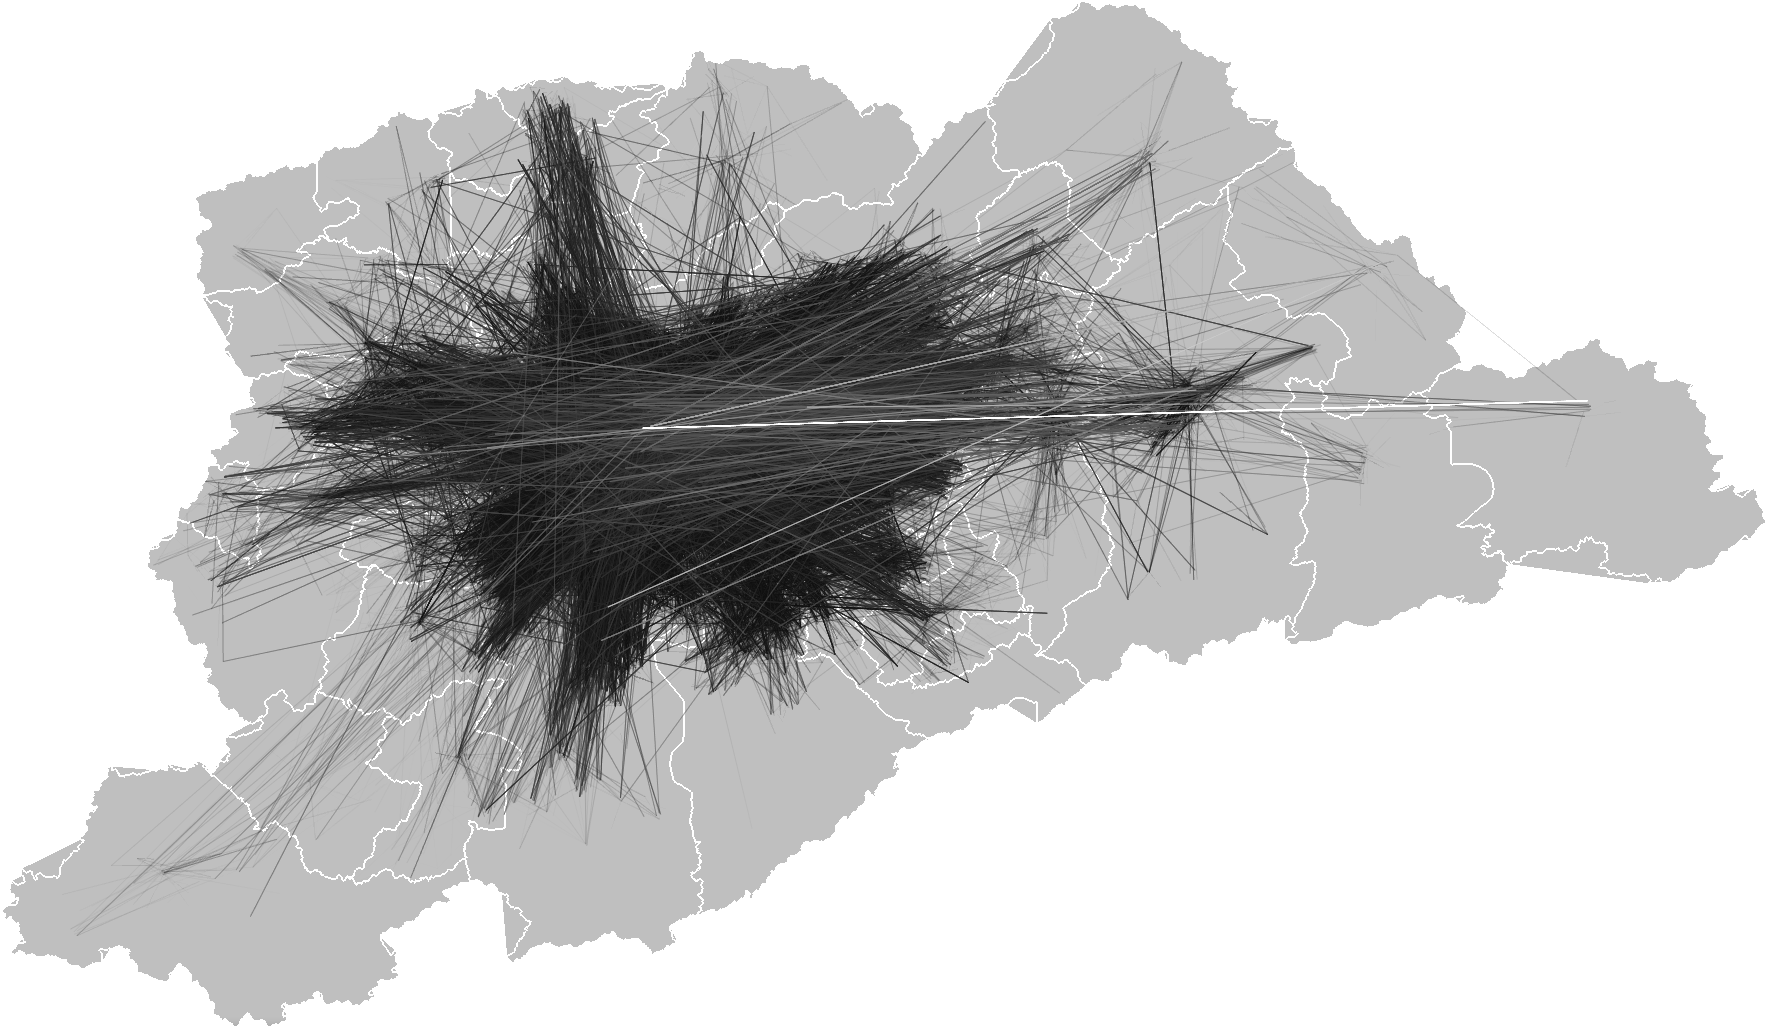
\includegraphics[width=150mm]{../figuras/unbundled-edges+grayscale+512px.png}
  \caption[Trajetórias da pesquisa OD na região metropolitana de S\~ao Paulo]{Trajetórias da pesquisa
OD na região metropolitana de S\~ao Paulo. \label{fig:cluttered-graph}}
  
\end{figure}

Neste trabalho nos propomos o uso de um conjunto de técnicas de visualização
para explorar as características de uma grande quantidade de dados de
mobilidade urbana. Para isso, nós adaptamos uma técnica que revelou resultados
interessantes na visualização de trajetórias em outros cenários como o do
tráfego aéreo e rastreamento do movimento da visão para o nosso contexto.
Nosso estudo permitiu a visualização dos dados em diferentes níveis de
granularidade espaço temporal, ajudando a encontrar padrões de mobilidade e
revelar novos insights a respeito do sistema de transporte de S\~ao Paulo e da
infraestrutura da cidade. Em contraste a outros trabalhos que utilizam técnicas
similares, nossa pesquisa ainda se destaca pela grande quantidade de dados
analisada. Para isso, apresentamos também uma metodologia para reduzir o tamanho
do conjunto de dados com impacto mínimo na sua significância estatística. 
